\chapter{EVENT RECOGNITION}
 \label{chap:eventrec}
It has been observed that the visual events are always modeled as stochastic temporal processes in the semantic space, basically the dynamic patterns of event is captured through collective evolution of the semantic concept. Hidden Markov Model (HMM) have always been favorite for the sequential pattern recognition. However, the HMM's have been struggled to incorporate both spatial and temporal context present in the event data.  In ~\cite{YanKe05}, event is treated as a space-time volume in the video sequence. Volumetric features based on optical flow are extracted for event detection which are commonly used in videos with single moving object (human) and action. In other work, complex activity recognition tasks are considered on internet videos which are already temporarily localized and they focus on localizing well defined primitive event~\cite{YanKe07}.
\par A common approach to video classification ~\cite{Liu09}~\cite{Niebles10} involves : extracting local region level features, combining features to fixed size video level description and trained a classifier on the features to predict the class labels. But in these approaches feature extraction plays a crucial role, hence features considered must be revisited for different sort of videos. Convolutional Neural Network(CNN) that replace all three stages with a single neural network ~\cite{Ji13} that is trained end to end from raw pixel values to classifier outputs. However we observe that the CNN are computationally expensive and requires a longer training period to effectively optimize but with improvements on GPU hardware have enabled CNNs to scale to networks of millions of parameters.
\par In section \ref{sec:cnn}  we will discuss the reasons on chosing the deep neural network for event recognition task while in section \ref{sec:pyDNN} elaborate the features that are supported by the indigenous neural network toolkit that was designed in python.s 
 \section{Convolutional Neural Network (CNN)}
 \label{sec:cnn}
 \par Covolutional neural networks (CNN) are variant of multi-layer perceptron (MLP) that are designed by studying the complex arrangement of cells in the cats visual cortex. It comprise of one or more convolutional layers (often with a subsampling step), followed one or more standard MLP.  Advantage of having CNN is that it learns faster (fewer parameters) compared to  MLP with the same number of hidden units. Just like normal MLP, CNN  also use  gradient based optimization to compute parameters of the model. It is  evident that CNN fits very well onto the visual recognition domain, as it handles very high dimensional data, exploits the topology of image or video and is invariant to small translation and illumination changes. 
CNN leverage following concepts to incorporate the above mentioned challenges,
\subsection{Local Connectivity}
It exploits the spatially local correlation by  allowing only local connectivity between neurons of adjacent layers. Hence, every hidden units is only sensitive to a small block in the visual field, called receptive field. This enable us to  drastically reduce the number of connections between input and hidden layer, which threfore diminishes the number of parameters needed to train the model.
\subsection{Shared Filters}
The hidden units are associated to the receptive field by filters which are shared within a feature map. These filters tries to capture edge like patterns within the receptive field. Additionally, sharing filters increases learning efficiency by greatly reducing the number of free parameters to be learned. Apart from reducing parameters, they extract the same feature at every position, which makes every feature map to be equi-variant to any changes in the input. The shared filters are associated to the receptive field by a dot product operation which can be expressed as a discrete convolution operation.
\subsection{Pooling/Sub-sampling Hidden Units}
According to this concept, we try to pool the hidden in non-overlapping neighbourhood. Among the techniques average and max pooling, max pooling has been commonly used as it provides local translation in-variance. Pooling also reduces inputs to next layer of feature extraction, thus allowing us to have many more feature maps. All feature maps in latter layer extracts coarser features.\par
All these concepts enable CNN to achieve better generalization in the vision problems. Stacking multiple such layers to attain better responsiveness over a larger visual field. Some architectural tricks such as rectification and contrast normalization, and using unsupervised pre-training of each filter weight also improves the robustness of the built models.
\section{Python-DNN Toolkit}
 \label{sec:pyDNN}
Neural networks can be best implemented using the modular, object-oriented approach. Where each models (dnn, sda, cnn) are implemented as a different class with following functions pre-train, fine-tune, test, load and save.



\subsection{Implementation}
Implementation of CNN is done in python using numerical computation library named \textit{Theano}. It provides platform to run efficiently in CPU and GPU architecture. Following are some key features of our implementation
\begin{itemize}
	\item  Allows easy configuration of the model, configurations are organized in JSON format thus makes the configuration legible to humans.
	\item Supports several types of data readers/writers.
	\item Enables us to dump CNN features for their use in other applications.
	\item Facilitates in loading pre-trained model and dumping the trained model.
	\item Supports two and three dimensional convolutional models.
	\item Run efficiently in CPU and GPU architectures.	
\end{itemize}
\begin{figure}[htpb]
   \begin{center}
	    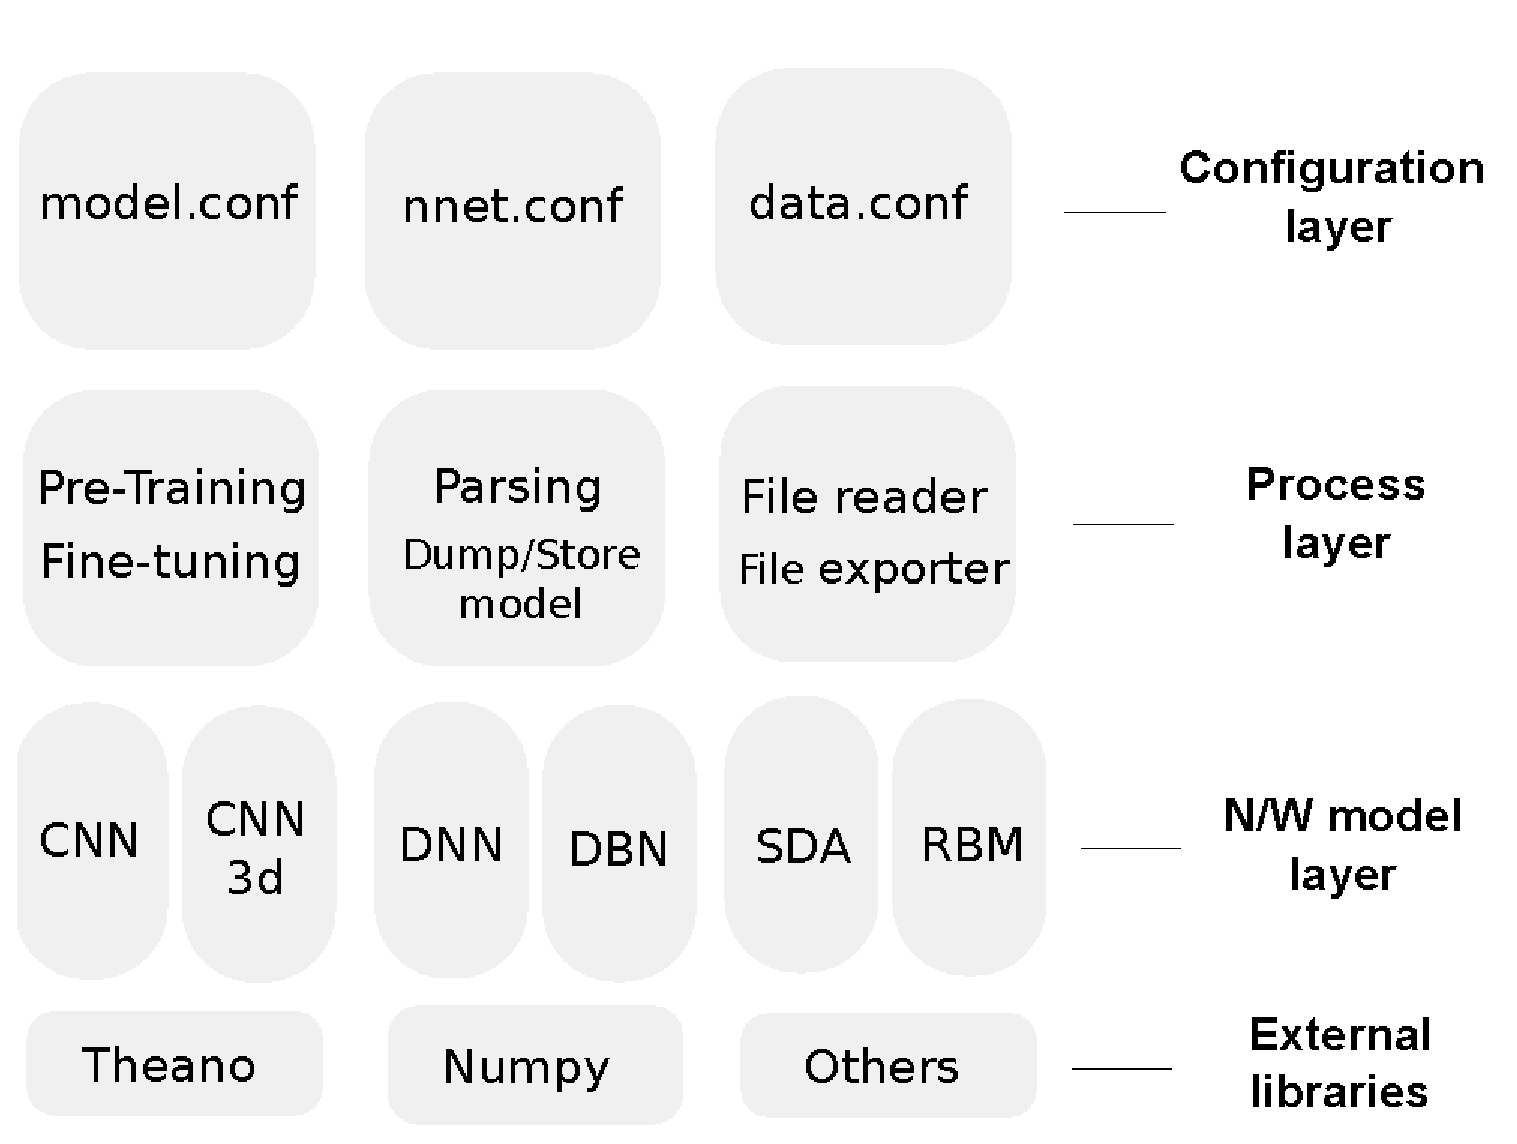
\includegraphics[width=0.75\textwidth]{snaps/architecture.eps}     
     \caption {Python-DNN Architecture}
	 \label{fig:architecture}
   \end{center}
 \end{figure}
\section{Summary}
Our implementation is publicly made available in github\footnote{\url{https://github.com/IITM-DONLAB/python-dnn}}. Architecture of the indigenous DNN toolkit is shown on \ref{fig:architecture}.Sample configurations for some well known dataset like MNIST and CIFAR are also made available with it.
The CNN is versatile, yet conceptually simple it has adapted to a wide spectrum of cognitive tasks. But training the CNN  requires a large number of labeled training samples. The CNN architecture takes advantage of the 2D structure of an input image (or spectrogram in case of speech signal) by the local connections and shared weights and provide translation invariance by subsampling the layer outputs.